% =============================================================================================
% paper/short/main.tex -- short version (8 pages of main text; references not counted) of the
% long paper paper/main.tex (git tag paper-v1, unchanged). Written from the v2 results
% (docs/PROTOCOL_v2.md, docs/STATUS_v2.md, docs/ROADMAP.md items D1-D3).
%
% Number sources (every number in the text and tables comes from one of these files):
%   [E1r] results_v2/tables/e1_size_real.tex        [E1s] results_v2/tables/e1_size_sim.tex
%   [E2s] results_v2/tables/e2_size.tex             [E2p] results_v2/tables/e2_power.tex
%   [E2d] results_v2/tables/e2dep_power.tex         [E2g] results_v2/tables/e2_dependent_size.tex
%   [E2b] results_v2/tables/e2_relative_boundary.tex
%   [E3]  results_v2/tables/e3_verdicts.tex, e3_power.tex, e3_stylized.tex  (10 seeds)
%   [E3'] results_v2_s50/tables/e3_verdicts.tex, e3_power.tex               (50 seeds, A2)
%   [E3L] results_v2/tables/e3_likelihood.tex, e3_likelihood_ag.tex, e3_agreement.tex
%   [E6]  results_v2/tables/e6_verdicts.tex, e6_stylized.tex; [E6'] results_v2_s50/tables/e6_verdicts.tex
%   [E7]  results_v2/e7tol/e7_curve.csv, results_v2_s50/e7tol/e7_curve.csv, e7_tolerance.tex
%   [E5]  results_v2/tables/e5_split.tex, e5_sensitivity.tex, e5_calibration.tex
%   [E4]  results_v2/tables/e4_correlation.tex, e4_utility_agg.tex, e4_link.tex, e4_placebo.tex
%   [v1]  paper/tables/e3_verdicts.tex (first protocol version, quoted once)
% Data/panel facts: paper/sections/data.tex. Theory: paper/sections/theory.tex (proofs in the
% long version's appendix).
%
% Compile from paper/short/:  latexmk -pdf main.tex
% Figure 1: from the repository root, uv run --project envs/gpu python paper/short/scripts/fig_tolerance.py
% =============================================================================================
\documentclass[11pt,a4paper]{article}

\usepackage[T1]{fontenc}
\usepackage{lmodern}
\usepackage{microtype}
\usepackage[margin=2.5cm]{geometry}
\usepackage{amsmath,amssymb,amsthm,mathtools,bm}
\usepackage[authoryear,round]{natbib}
\usepackage{booktabs}
\usepackage{graphicx}
\graphicspath{{figures/}}
\usepackage[font=small,labelfont=bf,skip=4pt]{caption}
\usepackage{xcolor}
\usepackage{hyperref}
\hypersetup{colorlinks=true, linkcolor=blue!50!black, citecolor=green!35!black,
            urlcolor=blue!60!black,
            pdftitle={Is Synthetic Financial Data Good Enough? (short version)}}
\usepackage[capitalise,noabbrev]{cleveref}

% Tighter space around floats (the article defaults are generous for an 8-page limit).
\setlength{\textfloatsep}{12pt plus 2pt minus 2pt}
\setlength{\floatsep}{10pt plus 2pt minus 2pt}

\theoremstyle{plain}
\newtheorem{proposition}{Proposition}
\crefname{proposition}{Proposition}{Propositions}

\newcommand{\todoinner}[1]{\textcolor{red}{\textbf{[TODO:}~#1\textbf{]}}}
\DeclareRobustCommand{\todo}[1]{\ifmmode\text{\todoinner{#1}}\else\todoinner{#1}\fi}

% --- Notation (same macros as paper/main.tex; meaning in paper/notation.md) -------------------
\newcommand{\E}{\mathbb{E}}
\newcommand{\Prob}{\mathbb{P}}
\newcommand{\W}{W_{1}}
\DeclareMathOperator{\Lip}{Lip}
\DeclareMathOperator*{\argmax}{arg\,max}
\DeclareMathOperator{\med}{med}
\DeclarePairedDelimiter{\norm}{\lVert}{\rVert}
\newcommand{\Gsig}{\mathcal{G}}
\newcommand{\dto}{\rightsquigarrow}
\newcommand{\TRAIN}{\textsc{train}}
\newcommand{\TEST}{\textsc{test}}
\newcommand{\Rpast}{R_{\mathrm{past}}}
\newcommand{\Rnew}{R_{\mathrm{new}}}
\newcommand{\Ppast}{P_{\mathrm{past}}}
\newcommand{\Pnew}{P_{\mathrm{new}}}
\newcommand{\QG}{Q_{G}}
\newcommand{\trn}{\mathrm{tr}}
\newcommand{\evl}{\mathrm{ev}}
\newcommand{\fhat}{\widehat{f}}
\newcommand{\ghat}{\widehat{g}}
\newcommand{\lgp}{\lambda_{\mathrm{GP}}}
\newcommand{\Danc}{\Delta}
\newcommand{\pmed}{p_{\mathrm{med}}}
\newcommand{\zhac}{z_{\mathrm{DK}}}
\newcommand{\GOOD}{\textsf{GOOD}}
\newcommand{\BAD}{\textsf{BAD}}
\newcommand{\INCONCL}{\textsf{INCONCLUSIVE}}
\newcommand{\INVALID}{\textsf{INVALID}}
\newcommand{\WC}{W-critic}
\newcommand{\GARCHt}{GARCH(1,1)-$t$}

\title{Is Synthetic Financial Data Good Enough?\\[0.3em]
  \large A Validated Critic Two-Sample Test with Likelihood Benchmarks and Markowitz Utility}
\author{\todo{Author names and affiliations}\thanks{Short version of a longer paper
  (\todo{reference}) that contains the proofs, the complete experiments and every table.
  Code, written protocol and its dated change log: \todo{repository URL}.}}
\date{Draft of \today}

\begin{document}
\maketitle

% [E1r] 0.05; [E1s] 0.095; [E3] GBM <0.001, D2 0.41; [E7] 0.92 (10 seeds), 0.995 (50 seeds).
\begin{abstract}
\noindent Synthetic asset returns are used to back-test strategies, share data and build
portfolios, but their quality is mostly judged by stylized facts or by scores without a null
distribution. We cast the question as a two-sample test with measured size and power. A
Wasserstein critic trained on half of the windows gives a held-out mean difference whose
permutation p-value is exact for independent windows. For dependent panels, a time-block split with
Driscoll--Kraay standard errors is asymptotically valid for a fixed critic; at nominal 5\% the whole
pipeline rejects a true null at 0.095 in a factor panel calibrated to the data, where splits by
stock reject at 0.93. Because markets change between
calibration and evaluation, the decision rests on an anchored relative test (is the generator
further from the new period than the real past is?) and on a power check that turns a
non-rejection into a certified tolerance. On 100 S\&P~500 stocks fitted on 2018--2022 and evaluated
on 2023 to mid-2025, geometric Brownian motion is rejected ($p<0.001$), whereas Merton, Heston,
GARCH-$t$ and a QuantGAN are not. The data cannot certify a 20\% volatility tolerance (rule power
0.41), but they certify 40\% against upward errors (power 0.92 with 10 synthetic seeds, 0.995 with
50), a reading chosen after the results were known and reported as such. In a Markowitz experiment,
the critic statistic does not predict the utility of portfolios built from synthetic data.
\end{abstract}

\noindent\textbf{Keywords:} two-sample test; Wasserstein critic; synthetic financial data;
relative similarity test; Driscoll--Kraay inference; power analysis; portfolio choice.
\textbf{JEL:} C12, C14, C45, C52, C58, G11.

% =============================================================================================
\section{Introduction}\label{sec:intro}

Synthetic returns, simulated from a fitted model or a trained generative network, are used to
back-test strategies on many paths instead of the single historical one
\citep{bailey2017probability}, to share data that cannot be disclosed \citep{assefa2020generating},
to train hedging strategies \citep{buehler2019deep} and to estimate portfolio inputs
\citep{cetingoz2026synthetic}. The generators range from geometric Brownian motion (GBM),
jump-diffusions, GARCH and stochastic volatility to generative networks
\citep{wiese2020quant,buehler2020data,ni2021sig}. Their quality is usually judged by comparing
stylized facts such as heavy tails and volatility clustering \citep{cont2001empirical}, or by
discriminative scores without a null distribution \citep{yoon2019time,stenger2024evaluation}.
Without a null distribution and a known power, a good score cannot be told apart from a weak
discriminator.

We treat the question as a hypothesis test. A defensible answer needs (i) level control on returns
that are serially and cross-sectionally dependent; (ii) known power against the deviations that
matter; (iii) a null that respects non-stationarity, since a generator calibrated on the past is
judged on a later period; and (iv) evidence on whether the answer predicts usefulness for a
decision. Our contributions follow this list.
(1)~A \emph{critic two-sample test with known level}: exact for independent windows, and for
dependent panels a time-block split with Driscoll--Kraay studentisation whose size we measure in
placebos calibrated to the data (\cref{sec:method-critic,sec:method-dep,sec:sim}).
(2)~An \emph{anchored relative test}, exact at its boundary, that asks whether a generator is
further from the evaluation period than the real past is, and a \emph{verdict with a certified
tolerance}: the smallest volatility error that the data can rule out with power 0.8
(\cref{sec:method-anchored,sec:method-verdict}).
(3)~A \emph{calibration} against the Neyman--Pearson oracle and five competing tests on simulated
windows with known laws (\cref{sec:sim}).
(4)~\emph{Evidence} on 100 S\&P~500 stocks for five classical generators and a neural one, with
likelihood benchmarks (\cref{sec:emp,sec:robust}), and on the Markowitz utility of portfolios built
from multivariate synthetic data (\cref{sec:mk}).

\paragraph{Protocol.} Settings, seeds, replication counts and the decision rule were fixed in a
written protocol before the runs reported here; later amendments are dated in its change log and
flagged in the text. Three choices were made with knowledge of earlier real-data results on the same
split: the time-pooled critic, adopted after a first protocol version with a perceptron critic; the
tolerance rule of \cref{sec:method-verdict}; and the increase from 10 to 50 synthetic seeds (both
are reported). The real-data verdicts are therefore not a blind confirmation.

\paragraph{Related work.} The statistic instantiates the held-out witness template
\citep{kirchler2020two,kubler2022witness} with a Wasserstein GAN critic
\citep{arjovsky2017wasserstein,gulrajani2017improved}; see also \citet{wang2022two,hu2026neural}. It
is a learned, sample-split relative of consistent specification tests
\citep{bierens1990consistent,corradi2005bootstrap}, with a different null: a generator fitted on one
period reproduces the window law of a later one. Relative similarity tests compare two candidates
with one reference \citep{bounliphone2016test,zhou_2025_anchor}; in ours one candidate is the real
past, as in forecast comparisons against a benchmark \citep{diebold1995comparing,giacomini2006tests}.
Two-sample tests have evaluated market generators \citep{buehler2020data,chevyrev2022signature}
without an analysis of their size and power on dependent data.

% =============================================================================================
\section{Method}\label{sec:method}

\subsection{Samples and the critic statistic}\label{sec:method-critic}

Daily log-returns $r_{it}$ of $N$ stocks are divided by the standard deviation $s_i$ of stock $i$'s
returns in the calibration period (\TRAIN), real and synthetic alike, and cut into non-overlapping
windows of $L=20$ days. Three samples are compared: the real windows of the evaluation period
(\TEST), $\Rnew=(X_1,\dots,X_n)$ with law $\Pnew$; windows simulated by a generator $G$ over the
same horizon, $(Y_1,\dots,Y_m)$ with law $\QG$; and the real \TRAIN{} windows,
$\Rpast=(Z_1,\dots,Z_k)$ with law $\Ppast$. The absolute null is $H_0:\Pnew=\QG$. It concerns the
law of one window, which fixes the dependence of returns up to lag $L-1$; dependence between
windows is a nuisance that the inference has to absorb.

Each sample is split into a training and an evaluation half. A critic $\fhat=\ghat\circ A$, where
$A$ standardises each coordinate with moments of the pooled training halves, is trained alone,
with no generator, on the gradient-penalised Wasserstein objective
\citep{gulrajani2017improved}
\begin{equation}\label{eq:wgan}
  \ghat\approx\argmax_g\big\{P^{\trn}(g\circ A)-Q^{\trn}(g\circ A)-\lgp\,\mathrm{GP}(g)\big\},\qquad
  \mathrm{GP}(g)=\E\big(\norm{\nabla g(\tilde x)}-1\big)^2,
\end{equation}
where $P^{\trn},Q^{\trn}$ are empirical means over the training halves and the penalty is taken at
$\tilde x=uA(X)+(1-u)A(Y)$, $u\sim U(0,1)$ ($\lgp=10$; Adam, learning rate $10^{-3}$, moments
$(0.5,0.9)$; 128 windows per sample and step; 1000 steps; no early stopping). The network $\ghat$ is a time-pooled convolutional critic: two
one-dimensional convolution blocks with 64 channels and kernel 5, an average over the days of the
window and a dense head of width 64. The statistic is the held-out mean difference
\begin{equation}\label{eq:T}
  T=\frac{1}{n_e}\sum_{i\in I_{\evl}}\fhat(X_i)-\frac{1}{m_e}\sum_{j\in J_{\evl}}\fhat(Y_j),
\end{equation}
one-sided, since the critic is trained to score real windows high.

\begin{proposition}[Target and exact level]\label{prop:exact}
Let $\Gsig$ be generated by the training halves, the split and the training randomness.
(a) If, given $\Gsig$, the evaluation windows have laws $P$ and $Q$, then
$\E[T\mid\Gsig]=P\fhat-Q\fhat\le\Lip(\ghat)\,\W(P_A,Q_A)$, the Wasserstein-1 distance between the
standardised window laws. (b) If the windows are i.i.d., the two samples independent, the split
independent of the window values and $H_0$ holds, the permutation p-value of $T$ computed with
$\fhat$ fixed satisfies $\Prob(p\le\alpha)\le\alpha$ for every critic, every number of permutations
and every sample size.
\end{proposition}

Part (b) is the randomisation principle \citep{hemerik2018exact}: a poor critic costs power, never
level. By (a), $T$ approximately lower-bounds $\W$; the penalty enforces the Lipschitz constraint
only softly, so $T$ serves as a test statistic, not as an estimate of $\W$
\citep{mallasto2019well}.

\subsection{Dependent windows}\label{sec:method-dep}

On real data the windows of a stock are dependent through volatility clustering, and windows of
different stocks on the same dates through common shocks. This breaks the permutation test in two
ways. Its variance ignores the dependence. Worse, if training and evaluation windows share dates,
the critic learns the realised volatility path of those dates, so $\E[T\mid\Gsig]>0$ under $H_0$;
a split by stock on common dates creates this bias in full, and no variance estimator can remove a
bias in the mean. We therefore cut the date range into $K=10$ blocks and assign whole blocks to the
training or the evaluation half, with labels shared across samples, so that training and evaluation
windows never share a date. $T$ is then studentised with the Driscoll--Kraay variance
\citep{driscoll1998consistent} of each sample. With $a_k=\fhat(X_k)$ on the evaluation windows and
date sums $\mathcal S_u=\sum_{k:u_k=u}(a_k-\bar a)$ on the grid of window start dates,
\begin{equation}\label{eq:dk}
  \widehat V(\bar a)=\frac{1}{n_e(n_e-1)}\Big[\sum_u\mathcal S_u^2
  +2\sum_{h=1}^{H}\Big(1-\frac{h}{H+1}\Big)\sum_u\mathcal S_u\mathcal S_{u+h}\Big],\qquad
  \zhac=\frac{\bar a-\bar b}{\sqrt{\widehat V(\bar a)+\widehat V(\bar b)}},
\end{equation}
with the Bartlett lag $H$ of the AR(1) plug-in rule of \citet{andrews1991heteroskedasticity}, and
p-value $1-\Phi(\zhac)$. Summing within a date absorbs arbitrary cross-sectional dependence.

\begin{proposition}[Validity for a fixed critic]\label{prop:dk}
If, given $\Gsig$, the evaluation windows are independent of the training data, their date sums
are strongly mixing with $2+\epsilon$ moments, and the Driscoll--Kraay estimators are consistent,
then $\zhac\dto N(0,1)$ under $H_0$ as the number of evaluation dates grows.
\end{proposition}

The blocks interleave without a gap, so the independence in \cref{prop:dk} holds only
approximately, and 15 evaluation dates make the variance estimate noisy: we measure the size of the
whole pipeline in placebos calibrated to the data (\cref{sec:sim}), with fixed-$b$ p-values
\citep{kiefer_2005_new} as a check. Kernel tests use a wild bootstrap with multipliers shared by
windows of the same date \citep{chwialkowski2014wild}.

\subsection{The anchored relative test}\label{sec:method-anchored}

A generator calibrated on the past inherits its features: in our data every generator fitted to
2018--2022 is more volatile than the 2023--2025 returns (\cref{sec:emp}). The absolute null asks the
generator to anticipate such changes, so its rejection does not separate a poor generator from a
change of regime. We therefore also compare $G$ with the naive benchmark of replaying history. One
critic is trained to separate all of $\Rnew$ (positive class) from an equally weighted pool of the
training halves of $G$ and $\Rpast$,
\begin{equation}\label{eq:anc}
  \ghat\approx\argmax_g\big\{\widehat P_{\mathrm{new}}(g\circ A)-\tfrac12\QG^{\trn}(g\circ A)
  -\tfrac12\Ppast^{\trn}(g\circ A)-\lgp\,\mathrm{GP}(g)\big\},
\end{equation}
and the statistic $\Danc=\Ppast^{\evl}\fhat-\QG^{\evl}\fhat$ compares its held-out means on past and
synthetic windows. $\Danc>0$ means that real past windows look more like the new period than
synthetic windows do: $G$ is worse than replaying history. For a shared critic the $\Rnew$ terms cancel,
$(\Pnew\fhat-\QG\fhat)-(\Pnew\fhat-\Ppast\fhat)=\Ppast\fhat-\QG\fhat$, which is why all of $\Rnew$
can be used for training.

\begin{proposition}[Level of the anchored test]\label{prop:anc}
(a) At the boundary $\QG=\Ppast$, if the three samples are independent and each is i.i.d., the
permutation test of $\Danc$ (labels of the held-out $G$ and $\Rpast$ windows permuted, $\fhat$
fixed) has level $\alpha$ in finite samples for every critic and whatever $\Pnew$. (b) Under the
conditions of \cref{prop:dk}, its Driscoll--Kraay version has asymptotic level $\alpha$ for the
null $\Ppast\fhat-\QG\fhat\le0$.
\end{proposition}

Differencing two separately trained critic statistics has no such guarantee: at this boundary its
size tends to $1/2$ for fixed critics and growing evaluation sets (long version). A generator that
resamples past windows, such as the stationary bootstrap, hands the test copies of windows the
critic saw, so the test is invalid for it.

\subsection{Verdict and certified tolerance}\label{sec:method-verdict}

An anchored p-value depends on the synthetic path and on the test randomness. With $S$ synthetic
seeds, each drawing both afresh, the verdict uses $\pmed=\min\{1,2\med(p_1,\dots,p_S)\}$, a valid
p-value under any dependence between the seed p-values \citep{meinshausen_2009_pvalues}. A non-rejection is evidence of quality only if the rule could have
detected a deviation of relevant size. A \emph{power check} simulates the whole rule, seeds
included, with the real sample sizes, dates and split, in two reference designs. D1 is a stationary
per-stock \GARCHt{} panel fitted on \TRAIN. D2 keeps the realised volatility path of \TRAIN{} (each
past window is its realised volatility times fresh Gaussian noise), uses the real \TEST{} windows as
$\Rnew$, and draws the boundary generator $G^0$ from the pooled law of the past windows. The
alternative multiplies the volatility of a synthetic draw by a factor $c$ (in D1 it also starts
from the end-of-\TRAIN{} state, the boundary from stationarity); let
$\beta_{\mathrm D}(c)$ be the rule power against it in design D. The pre-specified verdict, with
$\alpha=0.05$, is
\begin{equation}\label{eq:verdict}
  V=\begin{cases}
    \BAD & \text{if } \pmed\le\alpha,\\
    \GOOD & \text{if } \pmed>\alpha \text{ and } \min\{\beta_{\mathrm{D1}}(1.2),\beta_{\mathrm{D2}}(1.2)\}\ge0.8,\\
    \INCONCL & \text{otherwise.}
  \end{cases}
\end{equation}
When the rule cannot reach this tolerance of 20\%, we report the smallest one that the data can
certify: the smallest $t$ in a grid with $\beta_{\mathrm D}(1+t)\ge0.8$ and
$\beta_{\mathrm D}(1/(1+t))\ge0.8$ in both designs (amendment A1, written after the first verdicts
were known and before the runs it required). If the single-seed p-values are valid,
$\Prob(V=\BAD)\le\alpha$; if the true deviation is at least as detectable as the volatility error
of the designs, $\Prob(V=\GOOD)\le1-\beta$, where $\beta$ is the rule power. The second premise
cannot be verified and covers volatility errors only, so \GOOD{} means ``no detectable deviation of
the certified size and type'', never ``equal to the truth''. On real data the past is not
stationary and the first premise fails too, so the boundary size of the rule is estimated in D2 and
reported rather than assumed.

% =============================================================================================
\section{Size and power in simulation}\label{sec:sim}

\begin{table}[t]
\centering
\caption{Size: rejection rates under a true null at nominal 5\%. DK: Driscoll--Kraay p-value after
  the time-block split (conservative fixed-$b$ p-value in brackets); perm.: permutation after the
  same split; wild: wild bootstrap; KS: Kolmogorov--Smirnov on pooled returns (asymptotic; invalid
  under dependence). Independent windows: range over four families and $n\in\{500,2000\}$,
  permutation p-values (anchored: two boundary designs). One \GARCHt{} path: 500 consecutive windows
  per sample. Factor panel: the complete pipeline on a one-factor \GARCHt{} panel fitted to the
  data, synthetic stocks drawn jointly or independently. 200 replications (real placebo: 100).}
\label{tab:size}
\footnotesize
\setlength{\tabcolsep}{4pt}
% [E2s] [E2b] [E2g] [E1s] [E1r]
\begin{tabular}{@{}lcccccc@{}}
\toprule
 & \multicolumn{2}{c}{\WC{}} & Anchored & MMD & Sig-MMD & \\
\cmidrule(lr){2-3}
Setting & DK & perm. & DK & wild & wild & KS \\
\midrule
Independent windows & -- & 0.045--0.070 & 0.040--0.070 & 0.035--0.070$^a$ & 0.030--0.070$^a$ & 0.035--0.110 \\
One \GARCHt{} path & 0.080 & 0.190 & -- & 0.075 & 0.090 & -- \\
Factor panel, joint & 0.095 (0.045) & 0.505 & 0.120 (0.025) & 0.045 & 0.070 & 0.970 \\
Factor panel, indep. & 0.300 (0.230) & 0.535 & 0.185 (0.120) & 0.075 & 0.100 & 0.940 \\
Real placebo$^b$ & 0.05 (0.01) & 0.49 & -- & 0.33 & 0.38 & 0.46 \\
\bottomrule
\end{tabular}

\smallskip
\begin{minipage}{\linewidth}\footnotesize
$^a$ Permutation p-values. Wilson 95\% interval of a rate of 0.095 over 200 replications:
[0.062, 0.144].
$^b$ Random halves of the 100 stocks over the \TEST{} dates. The halves share dates and the
Driscoll--Kraay variance ignores their same-date covariance, so the critic's DK rates in this row
cannot reveal oversize; the wild bootstrap models that covariance.
\end{minipage}
\end{table}

\paragraph{Independent windows.} Four families of alternatives change the volatility level ($t_5$
windows), the tails ($t_\nu$ against $t_4$ at matched variance), the volatility clustering
(\GARCHt{} persistence) or the jumps (variance-matched GBM windows mixed into a Merton sample), with
$n=m$ windows of 20 days per sample. Under the null, the rejection rates of the five window tests
(\WC{}, a learned log-likelihood ratio or LR-critic \citep{cheng2022classification}, C2ST
\citep{lopezpaz2017revisiting}, MMD \citep{gretton2012kernel} and signature MMD
\citep{chevyrev2022signature}) lie between 0.025 and 0.095 over 40 cells of 200 replications, as
expected for exact tests up to Monte Carlo error (one of the 40 Wilson intervals excludes 0.05). KS
is not valid when the returns of a window share a conditional variance: it rejects at 0.110 in the
GARCH family with $n=500$.

\paragraph{Dependent windows.} Dependence breaks the permutation p-values, and the protocol of
\cref{sec:method-dep} repairs most of the damage (\cref{tab:size}). With consecutive windows of one
\GARCHt{} path, the \WC{} test rejects a true null at 0.265 with a random split and permutations,
and at 0.080 with the time-block split and Driscoll--Kraay variance. In a simulated factor panel
with the dimensions of our data, the complete pipeline rejects at 0.095 (fixed-$b$: 0.045; anchored
test: 0.120 and 0.025), against 0.930 for a split by stock with the same studentisation and 0.970
for KS. In a real-data placebo that compares random halves of the stocks, the wild-bootstrap kernel
tests reject at 0.33 and 0.38, although they were close to nominal in that panel (0.045 and 0.070):
real returns can be harder than a simulation calibrated to them. The largest gap appears when the
synthetic stocks are drawn independently, as univariate generators draw them: the absolute \WC{}
test then rejects a true null at 0.300 (anchored test: 0.185), so absolute rejections of univariate
generators are weak evidence.

\begin{table}[t]
\centering
\caption{Power at nominal 5\% with independent windows, $n=500$ windows of 20 days per sample, 100
  replications. The oracle is the Neyman--Pearson test with the true window densities (Monte Carlo
  integration over the starting variance for GARCH windows). $^\dagger$KS is oversized in this
  family (\cref{tab:size}).}
\label{tab:power}
\small
% [E2p] (a) 0.05, (b) 6, (c) 0.95, (d) 0.5; [E2d] window mixture k=2 (half i.i.d.), n=500.
\setlength{\tabcolsep}{5pt}
\begin{tabular}{@{}lccccccc@{}}
\toprule
Alternative & \WC{} & LR-critic & C2ST & MMD & Sig-MMD & KS & Oracle \\
\midrule
Volatility $\times1.05$ ($t_5$ windows) & 0.41 & 0.52 & 0.40 & 0.24 & 0.22 & 0.41 & 1.00 \\
Tails: $t_6$ against $t_4$ & 0.75 & 0.64 & 0.56 & 0.05 & 0.06 & 1.00 & 1.00 \\
Clustering: persistence 0.95 vs 0.98 & 0.56 & 0.57 & 0.58 & 0.26 & 0.28 & 0.89$^\dagger$ & 1.00 \\
Jumps: 50\% of windows from GBM & 0.14 & 0.07 & 0.14 & 0.07 & 0.06 & 0.34 & 1.00 \\
Dependence only: 50\% i.i.d.\ windows & 0.56 & 0.35 & 0.45 & 0.15 & 0.17 & 0.04 & 1.00 \\
\bottomrule
\end{tabular}
\end{table}

\paragraph{Power.} The exact oracle bounds the power of every two-sample test (for GARCH windows it
is a Monte Carlo approximation), and a mean-difference test with a fixed critic and a 50/50 split
has at most half the oracle's local noncentrality (long version), so a gap is expected.
\Cref{tab:power} shows it: at these deviations the oracle rejects in every replication, while the
best window test stays at 0.14--0.75. Against tails and jumps, KS on pooled returns is the most
powerful test, and any use of a window test has to be weighed against it. The critic is competitive
where a window test is needed: when only the dependence within a window changes and the marginal is
held exactly fixed, KS has no power (0.04) and the \WC{} test is the most powerful (0.56, against
0.15--0.45 for the others); it also beats the kernel tests against tails and clustering.

% =============================================================================================
\section{S\&P 500: verdicts and certified tolerance}\label{sec:emp}

\paragraph{Data and generators.} The data are daily closing prices of the 503 stocks in the S\&P~500
at extraction; 479 have a complete history and no data error, and the panel consists of 100 of them
drawn with a fixed seed. \TRAIN{} runs from 2018-01-03 to 2022-12-30 (1258 days) and \TEST{} from
2023-01-03 to 2025-06-16 (615 days), giving 6200 past and 3000 new windows. Five generators are fitted
per stock on \TRAIN: GBM, the Merton jump-diffusion, \GARCHt{}, Heston (quadratic-exponential scheme,
\citealp{andersen_2008_simple}) and the stationary bootstrap \citep{politis1994stationary}. A
QuantGAN \citep{wiese2020quant}, a temporal convolutional generator trained with a gradient penalty
on the pooled panel, was specified in the protocol before its first evaluation. Each generator
simulates one \TEST-length path per stock and seed, started from the fitted end-of-\TRAIN{} state
when the model has one. Every generator is more volatile than the evaluation period: the panel median
daily standard deviation of the six generators lies between 1.89\% and 2.13\%, against 1.62\% for
the real \TEST{} returns.
% [E3] stylized: 1.62 real; GBM 2.13, Merton 2.07, GARCH-t 1.89, Heston 2.06, bootstrap 2.05; [E6] QuantGAN 1.99.

\begin{table}[t]
\centering
\caption{Verdicts on the S\&P~500 panel. $\pmed=\min(1,2\times\text{median})$ of the seed p-values
  (Driscoll--Kraay); in brackets, the number of seeds whose absolute test rejects. Verdict: the
  pre-specified rule \eqref{eq:verdict}, which requires power against a volatility 20\% too high.
  Tolerance: smallest certified upward volatility error (directional reading, post hoc;
  \cref{fig:tol}); read as fixed, amendment A1 certifies $\pm100\%$ with 10 seeds. Rule power
  against $\times1.2$: 1.00 [0.98, 1.00] in D1; 0.41 [0.34, 0.47] (10 seeds) and 0.39 [0.33, 0.46]
  (50 seeds) in D2. Rule boundary size: 0.00--0.02 in both designs.}
\label{tab:verdicts}
\small
% [E3] [E3'] [E6] [E6']
\begin{tabular}{@{}lcccccc@{}}
\toprule
 & \multicolumn{2}{c}{Absolute \WC{}, $\pmed$} & \multicolumn{2}{c}{Anchored, $\pmed$} & Verdict & Tolerance \\
\cmidrule(lr){2-3}\cmidrule(lr){4-5}
Generator & 10 seeds & 50 seeds & 10 seeds & 50 seeds & at $+20\%$ & (upward) \\
\midrule
GBM & $<$0.001 (10) & $<$0.001 (50) & $<$0.001 & $<$0.001 & \BAD & -- \\
Merton & $<$0.001 (10) & $<$0.001 (50) & 0.436 & 0.098 & \INCONCL & 40\% \\
Heston & $<$0.001 (9) & $<$0.001 (49) & 0.560 & 0.122 & \INCONCL & 40\% \\
\GARCHt{} & $<$0.001 (6) & 0.019 (29) & 0.819 & 0.823 & \INCONCL & 40\% \\
QuantGAN & 0.042 (6) & 0.168 (24) & 0.265 & 0.766 & \INCONCL & 40\% \\
Stat.\ bootstrap & $<$0.001 (6) & 0.001 (30) & invalid & invalid & \INVALID & -- \\
\bottomrule
\end{tabular}
\end{table}

\paragraph{Verdicts.} The absolute test rejects every classical generator (\cref{tab:verdicts}), a
result we do not over-read given its oversize with independent synthetic stocks. The anchored test
rejects GBM only ($\pmed<0.001$ with 10 and with 50 seeds): GBM fitted to 2018--2022 is detectably
less like 2023--2025 than replaying 2018--2022, and it is \BAD. Merton, Heston, \GARCHt{} and
QuantGAN are not detectably worse than history; with 50 seeds \GARCHt{} (0.823) and QuantGAN (0.766)
are furthest from rejection, Merton (0.098) and Heston (0.122) closest. The rule is well calibrated
at its boundary (sizes 0.00--0.02), but in D2 it detects a volatility 20\% too high only with
probability 0.41 (0.39 with 50 seeds). No generator can be \GOOD{} at the pre-specified 20\%: all
four are \INCONCL{}.

\paragraph{Likelihood benchmarks.} GBM, Merton and \GARCHt{} have tractable likelihoods. Their
out-of-sample log-scores (2.566, 2.708 and 2.740 per day; pooled Amisano--Giacomini tests
\citep{amisano2007comparing} separate each pair with $p<0.001$) order them exactly as the pooled
critic statistic does (Kendall's $\tau=1$): the critic recovers the likelihood ranking without a
likelihood, and extends the comparison to Heston and QuantGAN, which have none.
% [E3L] e3_likelihood.tex (mean log-score, best ticker counts), e3_likelihood_ag.tex (pooled p),
% e3_agreement.tex (Kendall tau = 1 at seed 0 and for the median over seeds).

\begin{figure}[t]
\centering
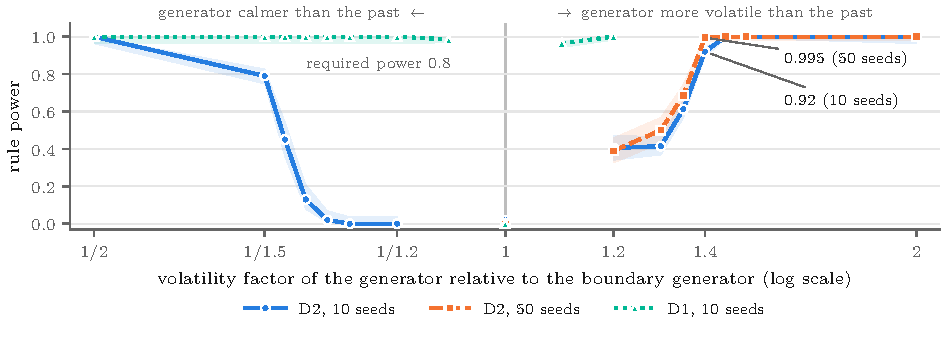
\includegraphics[width=\linewidth]{tolerance}
\caption{Power of the verdict rule (share of replications with $\pmed\le0.05$) against a generator
  whose volatility is multiplied by the factor on the horizontal axis, with Wilson 95\% bands
  (100--400 replications per point with 10 seeds, 200 with 50). At factor 1 the markers give the
  boundary size. D2 keeps the real 2018--2022 volatility path and uses the real 2023--2025 windows
  as $\Rnew$; D1 is a stationary \GARCHt{} panel, in which the alternative also differs from the
  boundary by its starting state. A calmer generator moves towards the calmer evaluation period,
  inside the anchored null in D2, so no power is expected there.}
\label{fig:tol}
\end{figure}

\paragraph{Certified tolerance.} \Cref{fig:tol} shows what the data can resolve. In D1 the rule
detects every factor measured, from $1/2$ to 1.2, with power at least 0.965, including $\pm10\%$. In
D2 the power against upward errors stays at 0.39--0.50 up to a factor 1.3, reaches 0.61 (0.685 with
50 seeds) at 1.35 and 0.92 [0.89, 0.94] (0.995 [0.972, 0.999]) at 1.4. Against downward errors the
D2 power is zero at factors $1/1.2$ and $1/1.3$ and reaches 0.79 only at $1/1.5$. This is expected:
\TEST{} was calmer than \TRAIN, so a too-calm generator is closer to the evaluation period than the
past is and lies inside the anchored null; requiring power against it was a mis-specification of
amendment A1. Read as fixed, A1 certifies only $\pm100\%$ (10 seeds; the 50-seed grid has no
downward cells). Dropping the D2 downward requirement certifies 40\% against upward errors, with 10
and with 50 seeds; this directional reading, and the finer grid of factors between 1.3 and 1.5 on
which it rests, were chosen after the first results were known. Merton, Heston, \GARCHt{} and
QuantGAN are thus not detectably worse than replaying history, within an upward volatility error of
40\%. The cut-off is sharp (0.685 at 35\%, 0.995 at 40\% with 50 seeds), and five times more seeds
do not move it, which points to the 615 days of a single evaluation period as the limit.
% [E7] 10 seeds: D1 min 0.965 at x1.1; D2 1.3 0.415, 1.35 0.6125, 1.4 0.92 [0.889, 0.943];
% 50 seeds: 1.3 0.50, 1.35 0.685, 1.4 0.995 [0.972, 0.999]; D2 down: 1/1.2, 1/1.3: 0.00; 1/1.5: 0.79.

% =============================================================================================
\section{Robustness}\label{sec:robust}

\paragraph{Sample split.} With calibration on 2018--2021 and evaluation from 2022-01-03 to
2025-06-16, the verdicts are unchanged (GBM \BAD; Merton, Heston and \GARCHt{} \INCONCL{}), but the
boundary size of the rule in D2 rises to 0.28 [0.16, 0.42], with power 0.36 [0.24, 0.50]. Under a
regime change between the periods, the rule can thus reject a generator that has exactly the past
law; controlling its size under such shifts is the main open problem.
% [E5] e5_split.tex

\paragraph{Critic settings.} We varied one setting at a time over 13 alternatives to the default:
window length 5, 10 or 60 days; critic width 32 or 256 channels instead of 64; 500 or 3000 steps;
learning rate $10^{-4}$; penalty weight 1; 4 time blocks; training fraction 0.3 or 0.7; and the
Newey--West lag rule, with 50 power replications each. GBM is \BAD{} in 10 of the 14
configurations; the exceptions are windows of 5 or 10 days, 500 steps and the lower learning rate.
Merton is \BAD{} in 4, Heston in 1 and \GARCHt{} in none. The D2 power against $\times1.2$ is 0.38
[0.26, 0.52] in 10 of the 13 alternatives, 0.44 with 4 blocks, 0.12 with a training fraction of 0.3
and 0.80 [0.67, 0.89] with 0.7, the only configuration in which a generator (\GARCHt{}) becomes
\GOOD{}; Merton and Heston are \BAD{} there. The resolution of the rule depends on how the data are
split, not on the network.
% [E5] e5_sensitivity.tex, e5_calibration.tex

\paragraph{Seeds and critic.} In the first protocol version (perceptron critic, 5 seeds), Merton and
Heston were \BAD{} ($\pmed=0.005$ and 0.017) and \GARCHt{} \INCONCL{} ($\pmed=0.432$). Near the
boundary, p-values move with the critic and with the number of seeds (Merton: 0.436 with 10 seeds,
0.098 with 50); hence we report both seed counts and a tolerance.
% [v1] paper/tables/e3_verdicts.tex

% =============================================================================================
\section{Does closeness predict portfolio utility?}\label{sec:mk}

The global minimum-variance (GMV) portfolio depends on the covariance matrix only up to scale, so a
generator whose only error is a volatility factor loses nothing for GMV, yet every consistent test
rejects it; conversely, an error in a low-variance direction, which GMV weights heavily, can be
almost invisible in $\W$ (long version). Closeness and usefulness can disagree in both directions.

We drew 30 universes of 30 stocks from the 479 and fitted five multivariate generators to each:
i.i.d.\ Gaussian and Student-$t$, CCC-\GARCHt, a stationary bootstrap of whole days and a one-factor
\GARCHt{} model. GMV and mean--variance portfolios \citep{markowitz1952portfolio} estimated from 20
synthetic samples of \TRAIN{} length were evaluated on the real \TEST{} period against the same
portfolios estimated on real \TRAIN{} returns. The average pairwise correlation fell from 0.419 in
\TRAIN{} to 0.268 in \TEST. Four generators give GMV portfolios whose \TEST{} variance is within 6\%
of the real-data portfolio's (variance ratios 0.954--1.054); the factor model loses most (1.436).
Within a generator, across universes, the multivariate critic statistic does not predict the GMV
variance ratio (Spearman $-0.10$ [$-0.32$, 0.13]); the distance between the synthetic and the past
average correlation does ($-0.36$ [$-0.52$, $-0.17$]), with a sign that reflects the fall in
correlations and need not hold when they rise. The multivariate critic test is also oversized in placebos for the
GARCH-type and bootstrap generators (0.17--0.45 at nominal 5\%, against 0.03--0.06 for the i.i.d.\
ones), a second open validity gap. Whether synthetic data are good for a task has to be checked on
that task.
% [E4] e4_correlation, e4_utility_agg (replica-wise GMV), e4_link (within-generator), e4_placebo.

% =============================================================================================
\section{Discussion and conclusion}\label{sec:concl}

The question in the title has a qualified answer. On this panel and split, GBM calibrated on
2018--2022 is not good enough: it is detectably further from 2023--2025 than the history it was
fitted to. Merton, Heston, \GARCHt{} and QuantGAN are not detectably worse than that history, within
an upward volatility error of 40\%; the pre-specified tolerance of 20\% cannot be certified with one
evaluation period of 615 days, and more synthetic seeds do not change this. Each verdict concerns a
model with its calibration on a period that contains the 2020 and 2022 turbulence, and one
pair of periods.

The size of the rule is not controlled under a regime shift (0.28 on the alternative split), and the absolute test over-rejects when synthetic stocks are
independent. The tolerance covers volatility errors only, and its directional reading, like the
critic architecture, was chosen with knowledge of earlier results on the same split. The panel
consists of index constituents at the end of the sample, a selection on outcomes beyond
survivorship bias \citep{brown1992survivorship}, and returns exclude dividends. A blind test on
returns after June 2025 under a protocol amendment fixed before the data are opened, and a
rolling-origin evaluation over several regimes, would turn these results into a confirmation. The
method itself (a critic test with measured size, a relative null anchored on the past and a
certified tolerance) applies to any generative model judged against a non-stationary reference.

\bibliographystyle{plainnat}
\bibliography{../references}

\end{document}
